\begin{equation}
Z(X) \overset{H_0}{\sim} N(0,1)
\end{equation}

A região crítica (4.3.5) é então definida (trocando $k_3$ em (4.3.5)) por $z_\alpha$ como
\begin{equation}
R_c = \left\{ x \in \mathcal{X} : \sqrt{n} \frac{\bar{x} - \mu_0}{\sigma} > z_\alpha \right\}
\end{equation}
\begin{equation}
= \left\{ x \in \mathcal{X} : Z(X) > z_\alpha \right\}
\end{equation}
em que $z_\alpha$ é tal que
\begin{equation}
P(Z > z_\alpha) = \alpha
\end{equation}

\begin{center}
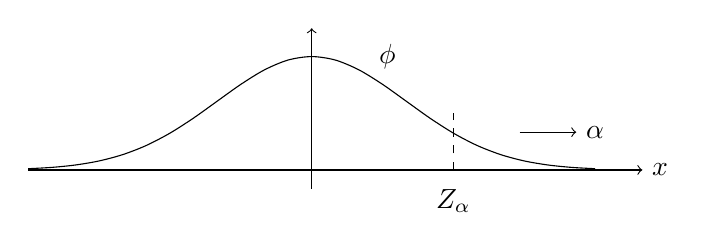
\begin{tikzpicture}[scale=1.2]
\draw[->] (-3,0) -- (3.5,0) node[right] {$x$};
\draw[->] (0,-0.2) -- (0,1.5);
\draw[domain=-3:3, smooth, variable=\x] plot ({\x},{1.2*exp(-\x*\x/2)});
\draw[dashed] (1.5,0) -- (1.5,0.6);
\draw (1.5,-0.1) node[below] {$Z_\alpha$};
\draw[->] (2.2,0.4) -- (2.8,0.4) node[right] {$\alpha$};
\draw (0.8,1.2) node {$\phi$};
\end{tikzpicture}
\end{center}

\section*{Resumo Teste Z}

\subsection*{Suposição}
$X_1, \ldots, X_n \overset{i.i.d.}{\sim} N(\mu, \sigma^2)$ e $\sigma^2 > 0$ conhecido.

\subsection*{Hipóteses}
\begin{equation}
\begin{cases}
H_0: \mu = \mu_0 \\
H_1: \mu = \mu_1 \ (> \mu_0)
\end{cases}
\end{equation}

\subsection*{Estatística de Teste}
\begin{equation}
Z(X) = \sqrt{n} \frac{\bar{x} - \mu_0}{\sigma} \overset{H_0}{\sim} N(0,1)
\end{equation}

